\chapter{System Design}  \label{chap:system-design}

This chapter details the system design of our Virtual and Distributed HSM, more specifically, the layers that compose our system and which contribute to its security in a distributed manner. It is followed by the system and adversary model, ending with an overview of the final architecture, where the roles and responsibilities of each component are described, as well as how they interact.

\section{Securing a Virtual HSM in a distributed way} \label{sec:securing-hsm}

A Virtual Hardware Security Module serves the same purpose as a physical HSM, but it exists only in the software environment and does not require any dedicated hardware to accomplish its normal cryptographic functionalities.

However, if we implement our system with only one server acting as a Virtual HSM, it would not be possible to achieve a similar level of security as a physical one since we would not have an isolated memory zone to protect sensitive data, such as keys, from the outside world; thus we would have a single point of failure that would certainly be an easy target for an attacker. Therefore, we had to implement our system in a distributed manner, and despite the difficulties and challenges this type of system causes, it allowed us to satisfy important properties, such as availability, integrity, and confidentiality.   

These properties are accomplished by combining several technologies and strategies in one system. Employing threshold cryptography protocols on top of a specific BFT SMR system allows us to develop a system with high availability, integrity, and confidentiality since if an adversary manages to compromise a replica, it would not reveal any information about the keys, nor would they be able to assemble the final result without compromising the other servers as well, which is very challenging to achieve. Moreover, the protocol and the system would keep functioning as expected due to the threshold strategy, where only a subset of the replicas are needed to conclude the operations, and even if an attacker tries to tamper with the system using counterfeit messages, the others can detect it by verifying the messages' integrity.

Furthermore, in order to implement a Virtual and Distributed HSM that aims to be practical and realistic, a BFT SMR system using a partially-synchronous communication model must be employed, since it is the classical approach for implementing consistent and fault-tolerant services. This approach maintains the integrity and availability of a secure service, even if a fraction of the replicas fail in a Byzantine way. As stated previously, our system was implemented on top of COBRA, which, besides the standard BFT SMR properties, also achieves data privacy, enabling us to take advantage of its features.


\section{System and Adversary Model} \label{sec:system-adv-model}

In terms of the system model, we consider a fully connected distributed system composed of a set of processes $\Pi$ divided into two non-overlapping subsets: a set of $n$ servers/replicas $\Sigma = \{s_1,s_2,..., s_n\}$, and an unbounded set of clients $\Gamma = \{c_1,c_2,...\}$. 
Clients access the system by requesting HSM operations, e.g., key generation, digital signature, and data encryption.

We assume a trusted setup in which each replica and client have a unique identifier that can be verified by every other process of $\Pi$ through standard means, e.g., a public key infrastructure. We suppress process IDs for readability when the processes involved are obvious. We further assume a partially synchronous model in which the network and processes may behave asynchronously until some \emph{unknown} global stabilization time ($\mathsf{GST}$), after which the system becomes synchronous, with \emph{known time bounds for computation and communication}. Finally, every pair of processes communicate through \emph{private and authenticated fair links}, i.e., messages can be lost and delayed, but not forever.

For the adversary model, we consider \textit{a probabilistic polynomial-time (PPT) adaptive adversary} that can control the network and may at any time decide to corrupt a fraction of the replicas in the current view. Replicas are allowed to deviate arbitrarily from the protocol, i.e., they are prone to Byzantine failures, and when corrupted, the adversary can learn the private state they store; however, if the failure threshold of each current view is respected, no confidential information can be obtained. More specifically, for a current view $\mathcal{V}$, the adversary can control simultaneously at most $\mathcal{V}.t = \lfloor\frac{\mathcal{V}.n - 1}{3} \rfloor$ replicas.

\section{Architecture Overview} \label{sec:arch-overview}

The high-level architecture of our system is illustrated in Figure \ref{fig:archvdhsm}, in which are represented two or more clients communicating with the system, specifically the servers that compose our virtual and distributed HSM, which exchange messages between themselves to resolve the received requests when it is needed. These requests are submitted by clients through the available Client API, which simplifies this process of requesting an operation by hiding all the necessary complexity underneath it. Ideally, clients would opt to use the PKCS\#11 API (also known as Cryptoki \cite{pkcs11spec}) to interact with the functionalities of a complete and standard HSM or the Crypto-Wallet API, which would be a simplified version of the Cryptoki API used by cryptocurrency wallets, that focuses basically on signatures and related features; however, we left these implementations for future work and implemented a simplified version that allows any client to interact with our system, and make use of the developed cryptographic operations. The specification of the Client API is described in the next subsection.


\begin{figure}[h]
    \begin{center}
        \resizebox{120mm}{!}{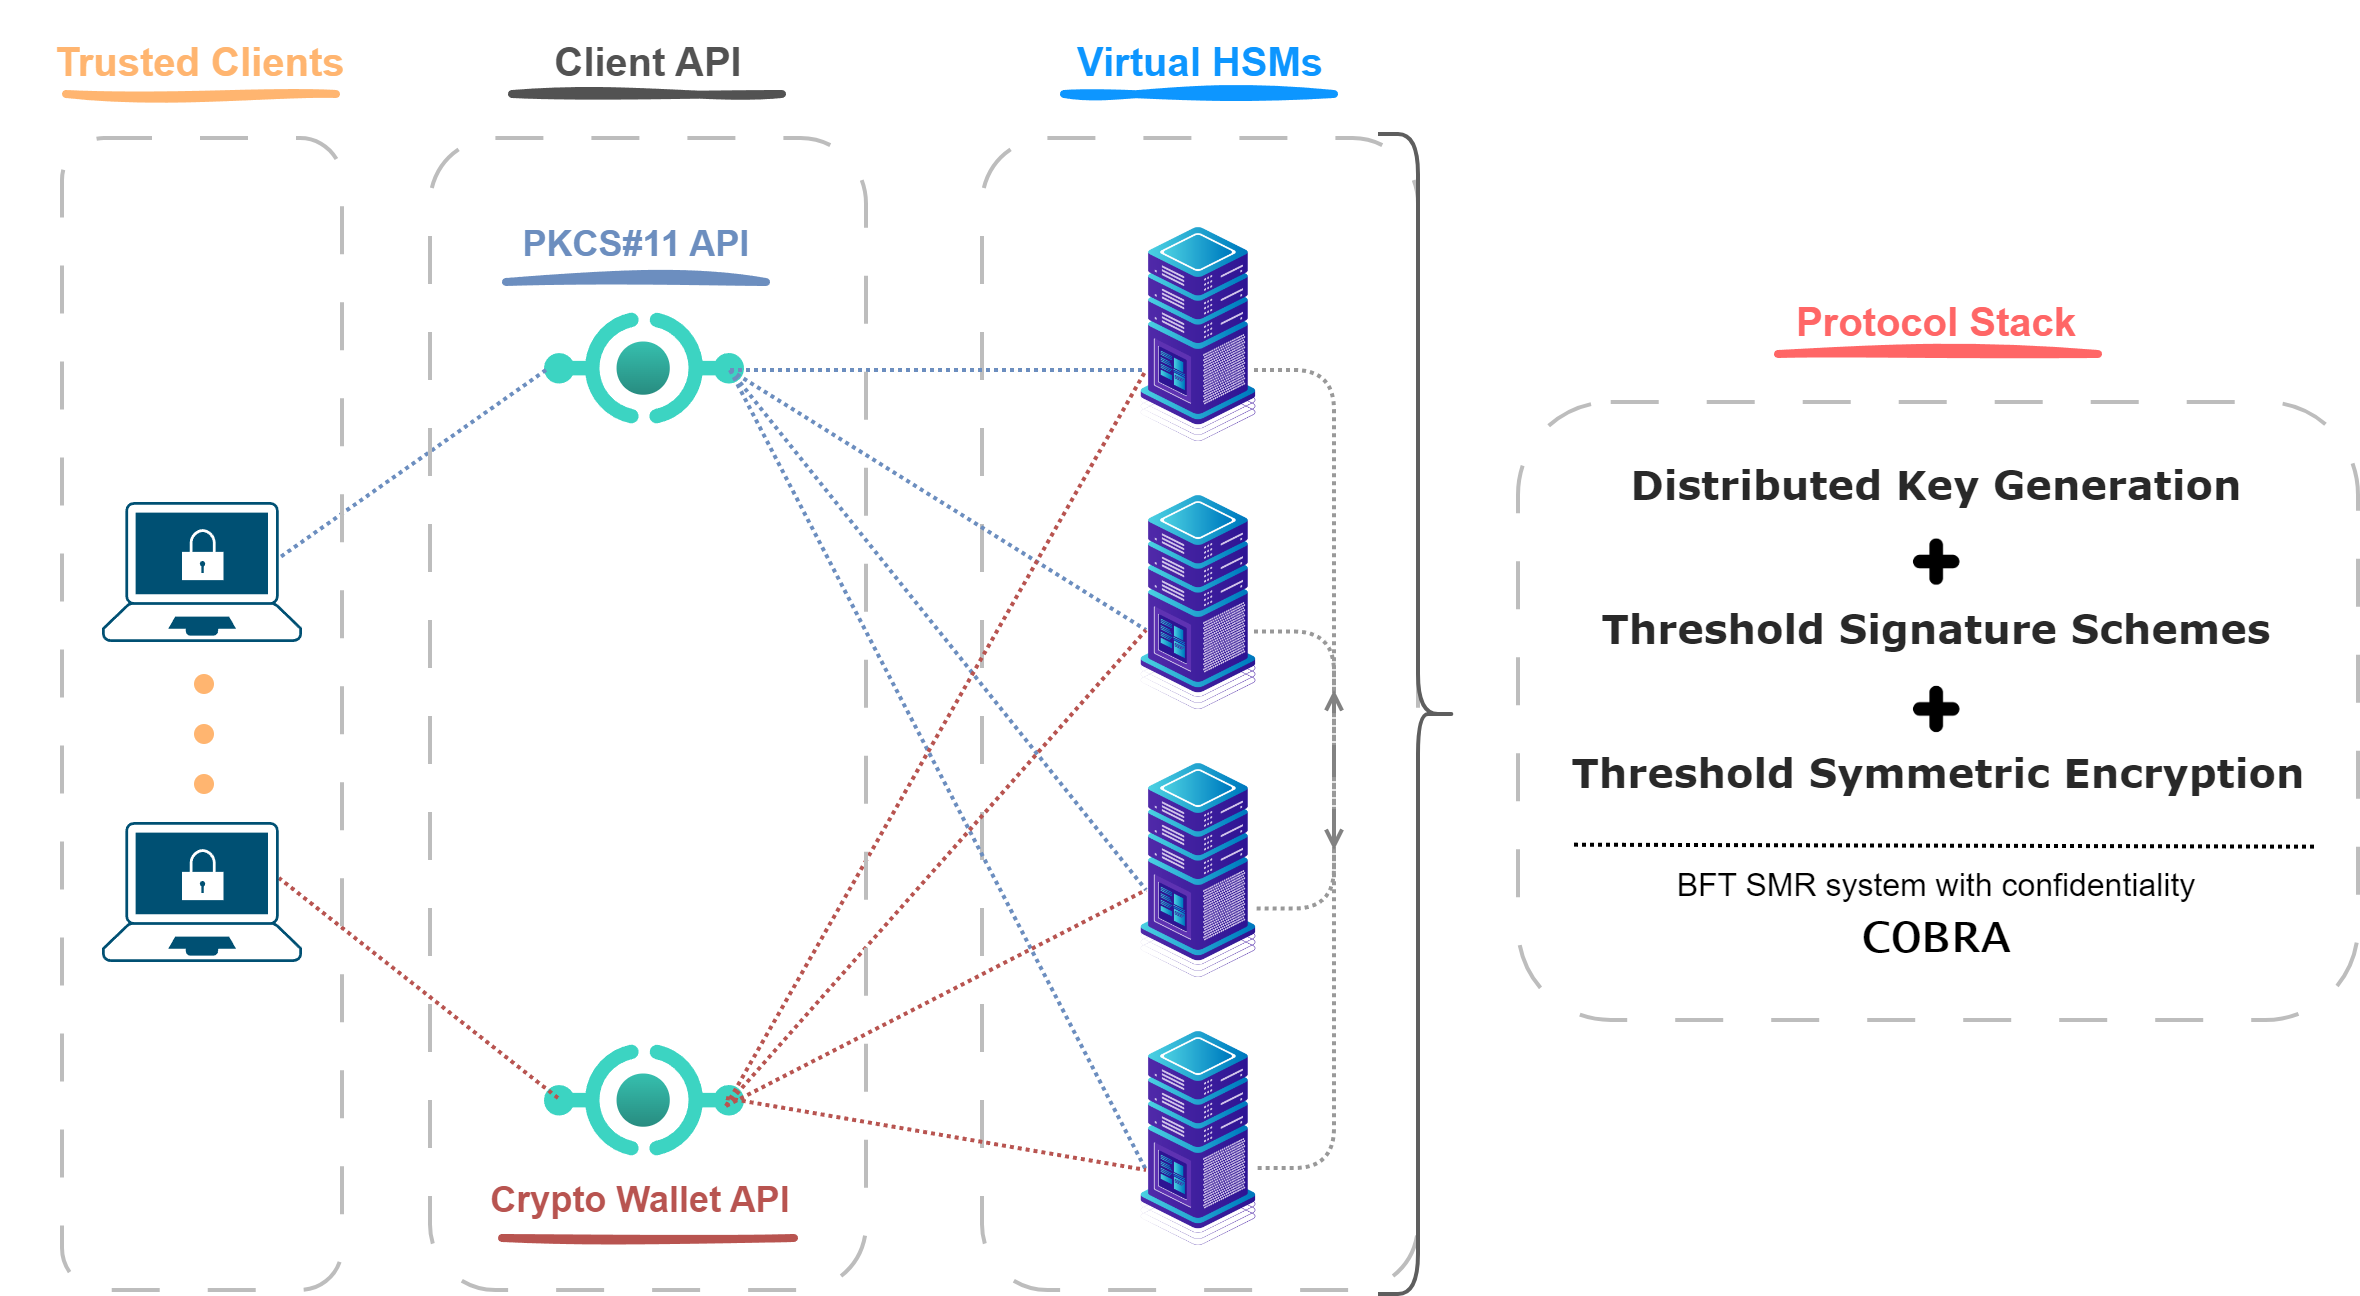
\includegraphics[]{4.system-arch}}
    \end{center}
    \caption{High-level architecture of our Virtual and Distributed HSM.}
    \label{fig:archvdhsm}
\end{figure}

Our system comprises the protocols that we have found to be the most efficient, secure, and practical since we were aiming for a system to be used in the real world. Our project's main algorithms correspond to a distributed key generation protocol, a threshold signature, and a threshold symmetric encryption protocol, as these are the distributed versions of the main features of a Hardware Security Module. Regarding the last two protocols, they follow a strategy where the replicas compute between themselves a partial result that each of them will send to the trusted client, which will be responsible for their aggregation into the final result, this being the signature or the final ciphertext. The protocols implemented in our Virtual and Distributed HSM are presented in the next chapter.

\subsection{Clients} \label{subsec:clients}
The clients are the system's entry point and must be trustworthy since they are responsible for initiating an operation and aggregating the partial results received into the final result. A compromised client would allow an attacker to manipulate the data sent to the servers, consequently enabling, for instance, the falsification of signatures or the decryption of any ciphertext previously issued by the same client. Hence, in our adversary model, we consider clients to be trusted.

To execute any of the available functionalities, a client needs to call the correspondent functions through the Client API, providing the required arguments depending on the feature being called.

The Client API covers and simplifies all the complexity of the implemented logic, making the available functionalities transparent to the final users. Specifically, it manages the encoding and decoding of messages sent and received from the servers, respectively, and the algorithms required for the partial results aggregation, which are exclusively produced by a specific set of the developed protocols, namely, signatures, encryptions, and decryptions.

The specifications of each of the functionalities available in the API are the following:
\begin{itemize}
    \item \texttt{generateKey(\textit{indexId}, \textit{keyScheme})$\longrightarrow$(success/$\perp$)}: Allows a client to submit a key generation request after providing the required arguments: \texttt{indexId}, i.e., a client unique index identifier that will be associated with the generated key that will act as a primary key in regular databases, allowing the client to select it or retrieve a previously generated \textit{public key}, in case of a asymmetric key pair, in the future; and \texttt{keyScheme}, a parameter that will allow generating the key for the correct finality, either selecting the proper elliptic curve for an asymmetric key generation (the currently available signature schemes are Schnorr and BLS schemes) or generating a symmetric key for the encryption operation. The result can either be a success message or $\perp$ if it was not possible to generate the requested key.
    
    \item \texttt{signData(\textit{indexId}, \textit{signatureScheme}, \textit{data})$\longrightarrow$(signature/$\perp$)}: Calling this function allows the client to issue a signature based on the provided arguments: \texttt{indexId}, the unique index identifier of the key to be used in the signature generation; \texttt{signatureScheme}, the scheme to be used when performing the signature, i.e., Schnorr or BLS, which must match with the one used in the selected key; and \texttt{data}, which corresponds to the data to be signed. In the end, the servers will respond with the issued signature or $\perp$, meaning that it was not possible to complete the signature protocol. Specifically, when successful, the client receives a pair containing the signature and the corresponding public key.

    \item \texttt{encryptData(\textit{indexId}, \textit{data})$\longrightarrow$(ciphertext/$\perp$)}: Function responsible for producing the encryption for the provided \texttt{data} using the key associated with the provided \texttt{indexId}. Returns the \textit{ciphertext} or $\perp$ if an error occurred and was not possible to finalize the encryption.

    \item \texttt{decryptData(\textit{indexId}, \textit{data})$\longrightarrow$(plaintext/$\perp$)}: Analogous to its encryption version, this function allows the decryption of the provided \texttt{data}, namely, a ciphertext previously generated by the encryption function using the key associated with the provided \texttt{indexId}. In the end, returns the initial \textit{plaintext} or $\perp$ in case it was not possible to conclude the decryption protocol.
\end{itemize}

The previously referred functions correspond to the most important ones since these implement the protocols studied in this project; however, the API still counts with some other utility functions:

\begin{itemize}
    \item \texttt{getPublicKey(\textit{indexId})$\longrightarrow$(\textit{publicKey}/$\perp$)}: Gets the \texttt{publicKey} associated with the private key that corresponds to the provided \texttt{indexId}. In case of an invalid or non-existent \texttt{indexId}, $\perp$ is returned.
    
    \item \texttt{validateSignature(\textit{signature}, \textit{publicKey}, \textit{data})$\longrightarrow$(\textit{Boolean})}: This function allows the verification of the validity of a produced \texttt{signature} using the correspondent \texttt{publicKey} and \texttt{data}, which is the data that was used to issue the signature in the first place. The function returns a \textit{Boolean}, specifically, \textit{true} if the signature was validated for the provided arguments or \textit{false} otherwise.

    \item \texttt{availableKeys()$\longrightarrow$(\textit{List<Keys>})}: Obtains from the servers the available keys the user requiring the operation has, returning a list of its keys, which specifically consists of the \textit{unique index identifiers}, the \textit{public keys}, and the \textit{signature schemes} used when generating each one of the stored keys.

    \item \texttt{commands()$\longrightarrow$(\textit{String})}: Client-side only operation that prints the available commands and how to use them properly.  
\end{itemize}


\subsection{Servers} \label{subsec:servers}
The servers are the most important component of our system since they implement the protocols that sustain the HSM service. Without them, we could not achieve the proposed objectives. 

Each server that composes our Virtual and Distributed HSM contains a stack of technologies that allow for the implementation of our distributed operations. Starting from the bottom layer, we have the library BFT-SMaRt \cite{bftsmart}, an implementation of a robust BFT SMR algorithm similar to PBFT \cite{pbft} that allows systems to extend and use its features, including state transfer for recovering a replica from a crash or slowness to the current state; reconfiguration of the set of replicas, allowing the addition or removal of replicas in runtime; and tolerance to faults, intrusions and asynchrony. The next layer is occupied by COBRA, a framework that implements confidentiality in BFT SMR systems using DPSS, particularly, extends BFT-SMaRt and adds on top of the previous features share recovery, secret resharing, and group reconfigurations without compromising the confidentiality of the stored secrets. The top layer, is where we implemented our cryptographic operations protocols. Our system takes advantage of all the features of the layers below, whether to ensure the security of secrets, making the system tolerant to intrusions, or simply using their communication manager to receive and respond to requests, all are extremely important to develop a practical and realistic system of this kind.

Basically, from a design point of view, upon receiving requests, the servers interpret them, execute the correspondent operation, and consequently, the matching protocol. Some operations require the servers to communicate with each other, being \textit{interactive}, while others are \textit{non-interactive}, meaning that the servers do not need to communicate between themselves to respond, each one only performs its own task and then send back the result to the client.

\begin{figure}[h]
    \begin{center}
        \resizebox{140mm}{!}{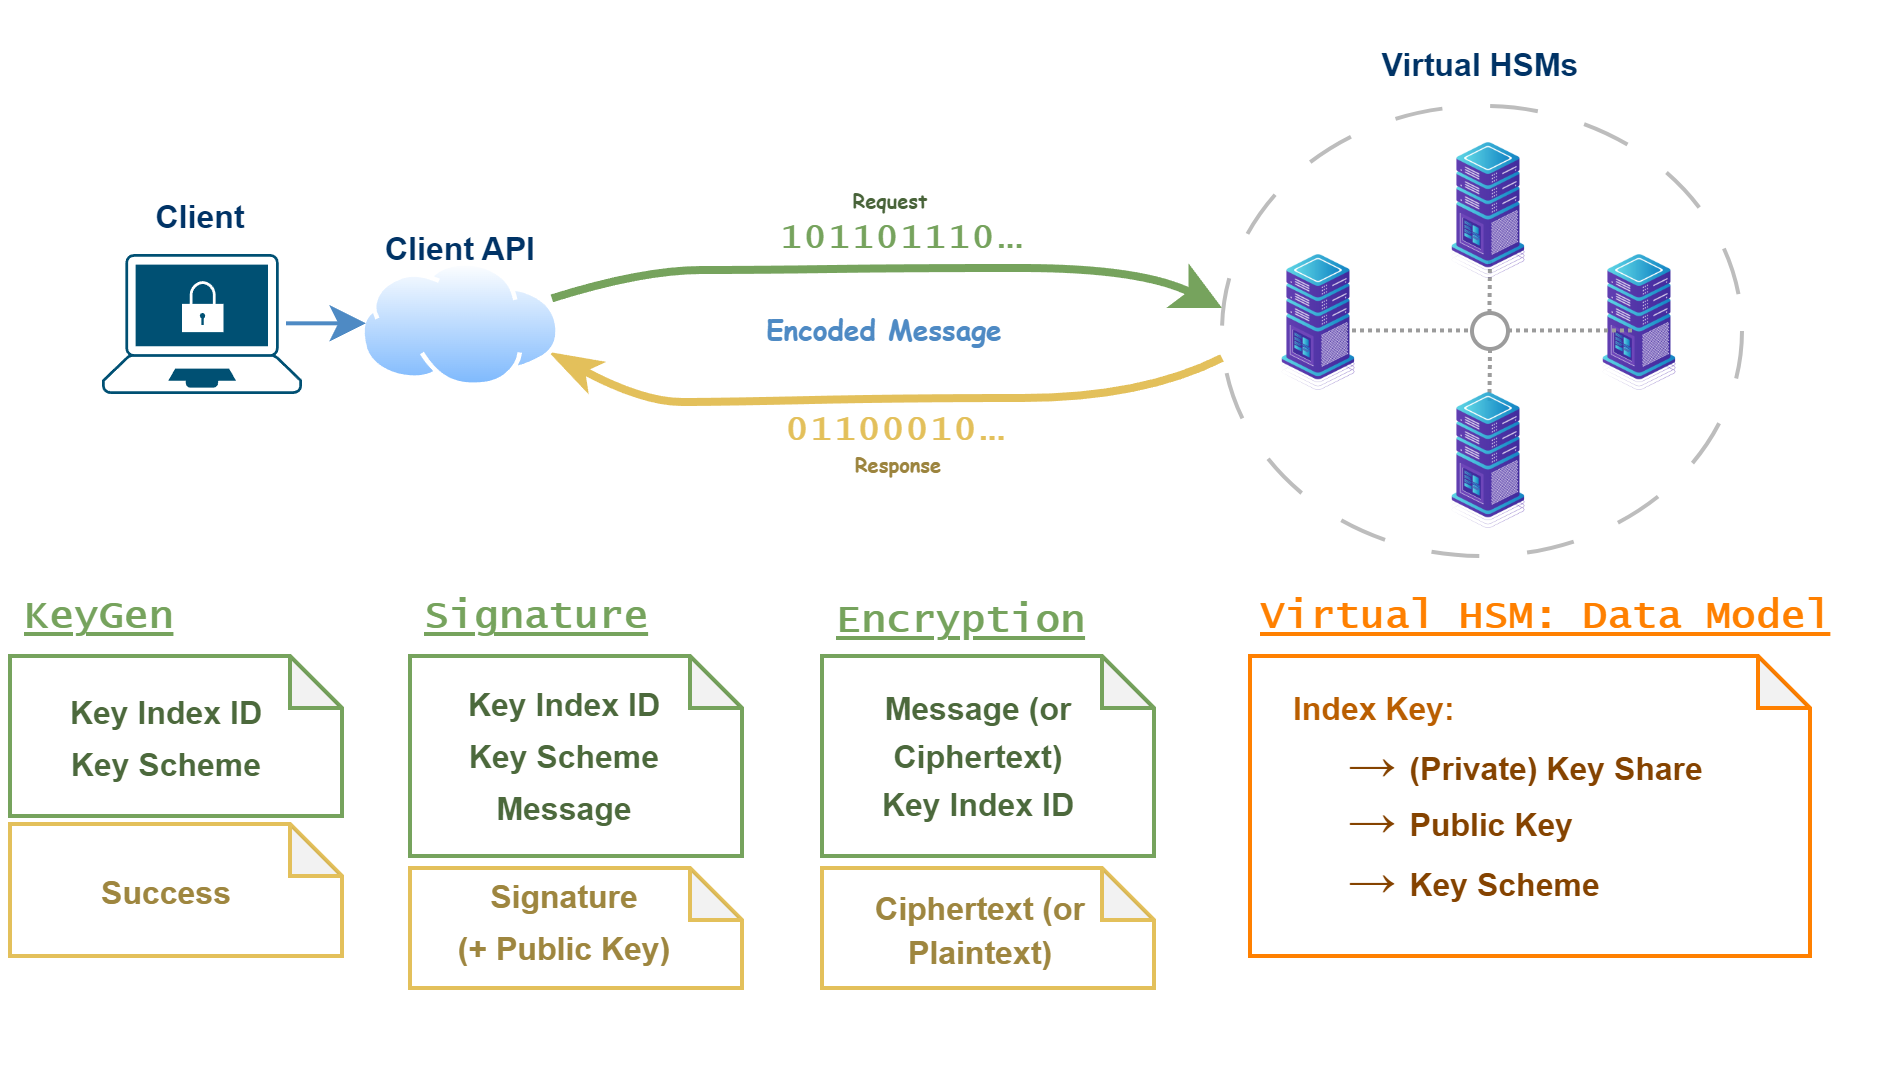
\includegraphics[]{4.data_model}}
    \end{center}
    \caption{Main operations and servers data model.}
    \label{fig:4.data_model}
\end{figure}

In addition to performing cryptographic operations, another main responsibility of our system, and HSMs in general, is safeguarding cryptographic keys. Each available server stores a share of the original private key, delivered by the Distributed Key Generation protocol to each one after the client requests the creation of a key. Specifically, each replica stores four different properties in its simple database (Figure \ref{fig:4.data_model}):
\begin{itemize}
    \item \textbf{Index Key}: A globally unique identifier, or primary key, associated with a generated key. This property allows clients to access their keys without conflicting with each other, because the identifier is composed of the \textit{client identifier} plus an \textbf{index identifier}, i.e., a client unique string submitted by the clients when requesting a key generation that will enable clients to distinguish between their stored keys;

    \item \textbf{Private Key Share}: Each replica stores a different portion of the generated private/secret key. The original key will never be reconstructed, and the shares will never leave their server;

    \item \textbf{Public Key}: To avoid spending time and resources to calculate a corresponding public key every time a client wants to retrieve one, we decided to store it alongside its corresponding private key;

    \item \textbf{Key Scheme}: The generated cryptographic keys are only compatible with a specific key scheme; therefore, we store that information to verify if the requested key scheme supports the provided key before starting the actual protocol. The available values that can be attributed to this property are \texttt{SCHNORR}, \texttt{BLS}, or \texttt{SYMMETRIC}.
\end{itemize}



\section{Final Remarks} \label{sec:design-final-remarks}

In this chapter, we discussed the design of our Virtual and Distributed HSM. Initially, we addressed the challenges of securing our system in a distributed manner, exposing how we achieve the most important properties that this type of system must have. All of those contribute to implementing a robust system that can prevail in a real-world environment. Next, we introduced the system and adversary model, presenting the assumptions made when implementing the project where the highlight goes to the clients, which we assume to be trustworthy. Therefore, the users are responsible for ensuring the security of their device, since it is there that the majority of the operations are completed. Afterward, we showed an overview of our system's architecture, followed by a description of the responsibilities of each major component, namely, clients, API, and servers. Specifically, we reveal the client's API end-users must follow when interacting with our system and the design of the data model implemented in the servers.  The next chapter discusses all the particularities of the system's cryptographic operations implementation.

% referir aqui que existem algumas funções que não requerem os servidores de comunicarem entre si, e dizer quais as operações e porquê 
%Regarding the servers' layers, there are some operations that do not require interaction between the servers due to their algorithm, namely, performing a BLS signature or an encryption/decryption. When these operations are received by the servers,  

%\LIMPA